\documentclass[tikz]{standalone}

\usetikzlibrary{calc}
\usetikzlibrary{decorations.pathmorphing,patterns,decorations.markings,arrows.meta,intersections}


\tikzset{
  cross/.style={
    path picture={
      \draw[thick]
        (path picture bounding box.south east) -- (path picture bounding box.north west)
        (path picture bounding box.south west) -- (path picture bounding box.north east);
    }
  }
}


\tikzset{
    angle bracket base/.style 2 args={
        to path={
            -- ($(\tikztostart)!0.5!(\tikztotarget)!#1!#2:(\tikztotarget)$) -- (\tikztotarget)
        }
    },
    angle bracket/.style={angle bracket base={#1}{90}},
    angle bracket/.default=0.4cm,
    angle bracket flipped/.style={angle bracket base={#1}{-90}},
    angle bracket flipped/.default=0.4cm
}

%set coordinates that randomly perturbes the original path
\tikzset{set random waves/.style args={#1and#2with name #3}{postaction={decorate,decoration={markings,
mark=at position 0.1 with {\coordinate[xshift={rand*#1},yshift={rand*#2}] (#3-1);},
mark=at position 0.2 with {\coordinate[xshift={rand*#1},yshift={rand*#2}] (#3-2);},
mark=at position 0.3 with {\coordinate[xshift={rand*#1},yshift={rand*#2}] (#3-3);},
mark=at position 0.4 with {\coordinate[xshift={rand*#1},yshift={rand*#2}] (#3-4);},
mark=at position 0.5 with {\coordinate[xshift={rand*#1},yshift={rand*#2}] (#3-5);},
mark=at position 0.6 with {\coordinate[xshift={rand*#1},yshift={rand*#2}] (#3-6);},
mark=at position 0.7 with {\coordinate[xshift={rand*#1},yshift={rand*#2}] (#3-7);},
mark=at position 0.8 with {\coordinate[xshift={rand*#1},yshift={rand*#2}] (#3-8);},
mark=at position 0.9 with {\coordinate[xshift={rand*#1},yshift={rand*#2}] (#3-9);}
}}}}


\tikzset{
arrow at/.style 2 args={postaction={decorate,decoration={
    markings,
    mark=at position #1 with {\arrow{Stealth[#2]}}
  }}},
}



\begin{document}
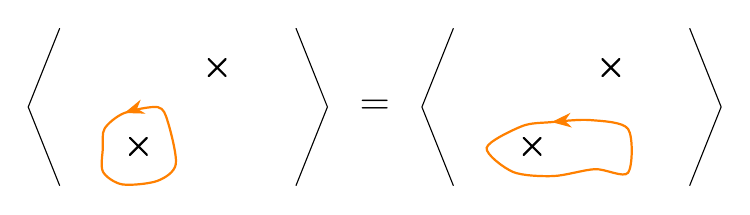
\begin{tikzpicture}
\begin{scope}
% brackets
\draw (0,-1) to[angle bracket] ++(0,2);
\draw (3,-1) to[angle bracket flipped] ++(0,2);

% operator insertions
\node[cross, minimum size=1] at (2,.5) {};
\node[cross, minimum size=1] at (1,-.5) {};



\pgfmathsetseed{1}
\path[set random waves=0.1cm and 0.1cm with name mypath] (1,-.5) circle (0.5cm);
\draw[smooth, orange,thick,-{Stealth[red]},save path=\pathA] plot[smooth cycle] coordinates {(mypath-1) (mypath-2) (mypath-3) (mypath-4) (mypath-5) (mypath-6) (mypath-7) (mypath-8) (mypath-9)};
%\draw[blue, ->][use path=\pathA];

%\path[arrow at={1.0}{red}] (mypath-1) to[out=45,in=135] (mypath-2);
\path[arrow at={.99}{orange,length=.25cm}] (mypath-1) to[out=45,in=20] (mypath-3);


\end{scope}

\node at (4,0) {\Large $=$};

\begin{scope}[xshift=5cm]
% brackets
\draw (0,-1) to[angle bracket] ++(0,2);
\draw (3,-1) to[angle bracket flipped] ++(0,2);

% operator insertions
\node[cross, minimum size=1] at (2,.5) {};
\node[cross, minimum size=1] at (1,-.5) {};

\pgfmathsetseed{2}
\path[set random waves=0.1cm and 0.1cm with name mypath] (1.5,-.5) ellipse [x radius=1cm,y radius=.4cm];
\draw[smooth, orange,thick,-{Stealth[red]},save path=\pathA] plot[smooth cycle] coordinates {(mypath-1) (mypath-2) (mypath-3) (mypath-4) (mypath-5) (mypath-6) (mypath-7) (mypath-8) (mypath-9)};
%\draw[blue, ->][use path=\pathA];
\path[arrow at={.99}{orange,length=.25cm}] (mypath-1) to[out=90,in=5] (mypath-3);

\end{scope}
    
\end{tikzpicture}
\end{document}
